\documentclass[letterpaper,12pt]{article}

\usepackage{mathpazo}
\usepackage[longnamesfirst]{natbib}
\usepackage[flushleft]{threeparttable} 
\usepackage{booktabs}
\usepackage{rotating} 
\usepackage{amssymb} 
\usepackage{amsmath}
\usepackage{caption} 
\usepackage{dcolumn} 
\usepackage{setspace}
\usepackage[longnamesfirst]{natbib}
\usepackage[font=scriptsize]{subfig}
\usepackage[pdftex,colorlinks=true,linkcolor=black,citecolor=black]{hyperref} 
\usepackage[margin=1.0in]{geometry} 
\usepackage{multirow}

\newcommand{\mco}[1]{\multicolumn{1}{c}{#1}}
\newcommand{\mct}[1]{\multicolumn{2}{c}{#1}}


%opening
\title{Fertility Issues in Developing Countries} 

\author{Claus C P\"ortner\\
    Department of Economics\\
    Albers School of Business and Economics\\
    Seattle University, P.O. Box 222000\\
    Seattle, WA 98122\\
    \href{mailto:cportner@seattleu.edu}{\texttt{cportner@seattleu.edu}}\\
    \href{http://www.clausportner.com}{\texttt{www.clausportner.com}}\\
    \& \\
    Center for Studies in Demography and Ecology \\
    University of Washington\\ \vspace{2cm}
    }

\date{February 2017}

\doublespacing

\begin{document}
\graphicspath{{../figures/}}
\DeclareGraphicsExtensions{.jpg,.jpeg,.pdf,.mps,.png}

\maketitle
\thispagestyle{empty}


\newpage

\section{Introduction}

Despite a common perception that fertility is very high in developing countries,
the truth is substantially more complicated.
Figure \ref{fig:TFR} shows that there has been an astonishing decline in total 
fertility rate (TFR) in developing countries over the last half century.%
\footnote{
TFR is the number of children a women entering her reproductive life
would have if she had children following the age-specific fertility
rates observed at that point in time.
Hence, it is composite or snapshot measure of current fertility
behavior.
}
Half a decade ago, TFR was around 7 children, with the exception
of TK.
The most recent data show, however, that, with the exception of 
Sub-Saharan African, TFR is now either below or only slightly 
above the replacement level of 2.1.
Despite this rapid decline in fertility population size is still
growing in many of these regions because there are still many
more young people than older people and these young people either
have not entered reproductive age or are just starting out.

\begin{figure}[hp]
    \centering
    \caption{Total Fertility Rates by Region from 1967 to 2015}
    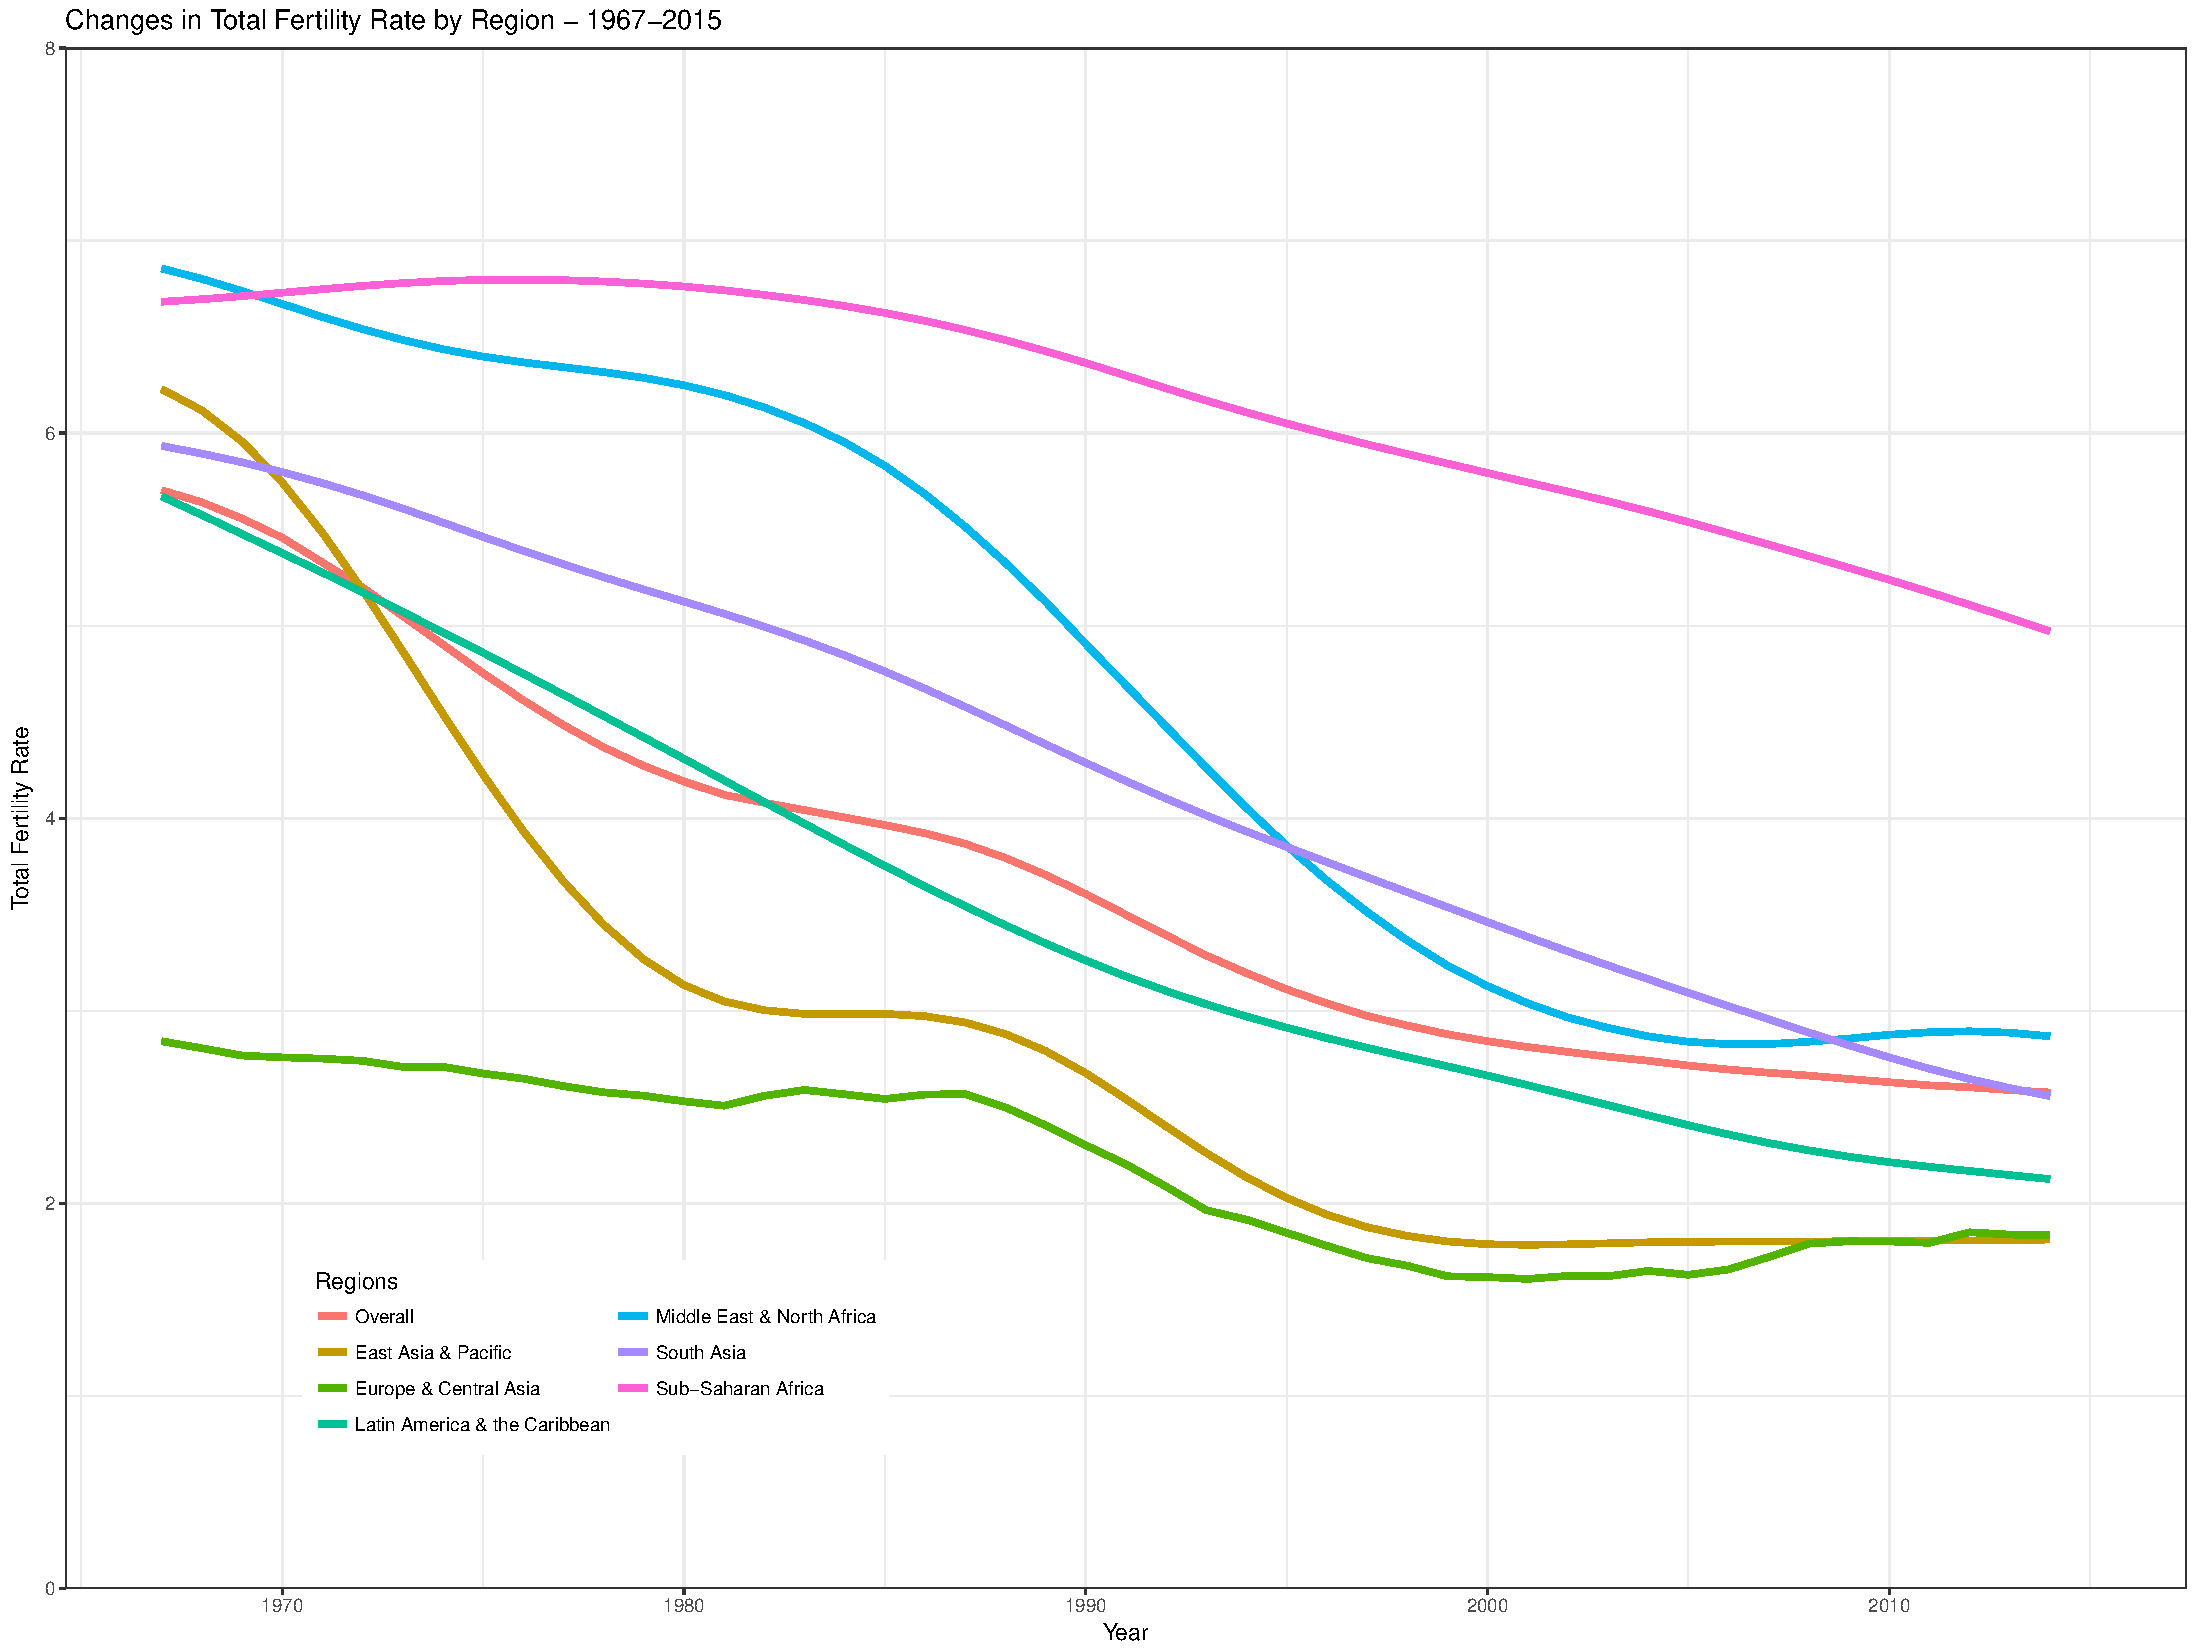
\includegraphics[width=0.75\linewidth]{totalFertilityRates}
    \label{fig:TFR}
\end{figure}

If fertility levels are close to identical across developing and
developed countries and there is rapid urbanization and increasing
labor force participation among women do we even need a developing 
country version of this chapter?%
\footnote{
TK references on urbanization and labor force particpation.
}
The goal of this chapter is to highlight where and why a
separate focus on developing countries is still relevant,
what the recent developments in research has been, and
most importantly, what I consider to be the main
outstanding issues.

The most important issues from a policy standpoint is why the 
fertility decline in Sub-Saharan Africa have moved at a much
slower pace than the other regions.
Sub-Saharan Africa now has an average TFR that is about twice
as large as the other regions.


\section{Sub-Saharan Africa}

The one outlier in the figure above is Sub-Saharan Africa. 

\cite{Gerland2014}


\section{Timing of Fertility}

As the figure above shows 


\citet{Dupas2017}


\section{Intrahousehold Allocation}

\cite{merli00} on missing girls in China


\section{Conclusion}


\bibliographystyle{aer}
\bibliography{collection}


\end{document}
